%% ------------------------------------------------------------------------- %%
\chapter{Introduction}
\label{cap:Introduction}

One of the most used data structures in computer science are dictionaries, which are also known as associative array, map or symbol table. Those are a collection or key-value pairs, where all pairs have different keys. The data structure supports the operations of inserting a new pair, finding the value associated to a given key, and deleting a pair. If one thinks about it, this is perhaps one of the most executed tasks in many software systems. For instance, the call history of numbers on a cell phone shows for each phone number, the owner of that number. In a dictionary we can insert a phone number and its owner, so that given a phone number one can retrieve the owner. 


\begin{figure}[h!]
  \centering
  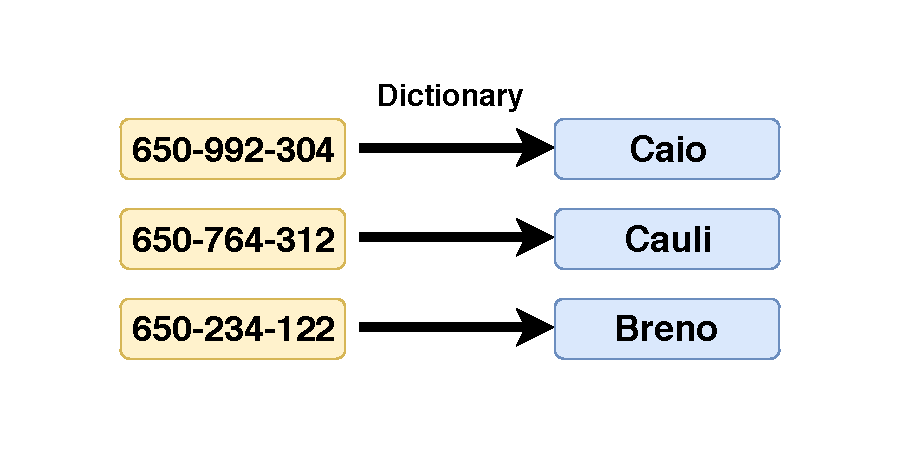
\includegraphics[width=12cm]{figuras/dictionary-example.pdf}
  \caption{Example of a dictionary that associates phone numbers to contact names. }
\end{figure}

Other use of a dictionary that we can think is to count the frequency that a certain number was called. One of the most common and efficient implementations of dictionaries is with a hash table. A key component in the implementation of a hash table is a hash function. This function usually takes the key of the key-value pair we want to insert, find or delete in the table and ``digest'' it into a number. That number is then used to identify the value, in this structure that we call hash table. In our example, the keys are phone numbers and the values are contact names.

An example of a hash function, that ``digest'' the phone numbers is the following: \\

\bigskip

\begin{figure}[h!]
  \centering
  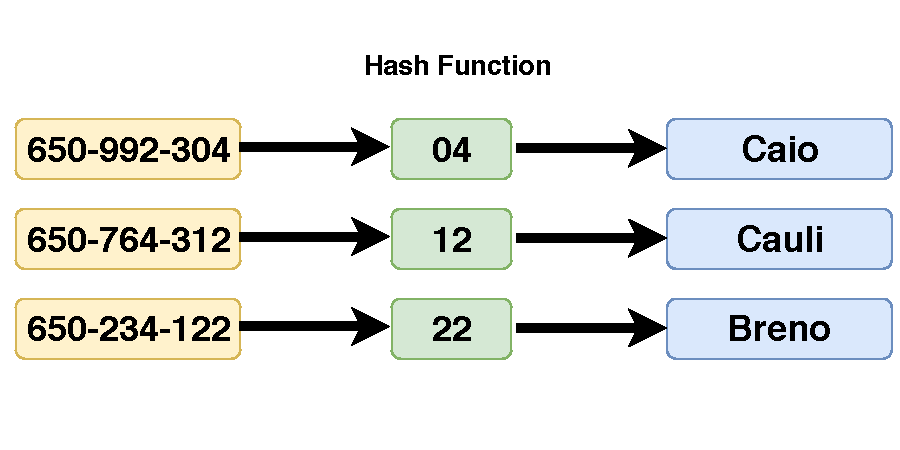
\includegraphics[width=12cm]{figuras/phone-hash-example.pdf}
  \caption{Example of a hash function that just takes the last 2 digits of the phone number }
\end{figure}

\medskip

As you can see this is a pretty simple function, it simply take the last 2 digits of each phone number. In this specific case, this is enough to uniquely identify each phone. We can imagine a function that can't uniquely identify each phone number, like getting just the last digit, in this case, Cauli's and Breno's numbers would have the same hash value, a collision in the table. Handling collisions in a hash table is a complete topic by itself, and it will be addressed in Chapter 3. 

Handling collisions is actually a very important topic in hash tables as the vast majority of hash functions will have collisions. To illustrate this situation we recall the ``Birthday Paradox'', that states that we only need 23 people in a room to have a chance greater than \( 50\% \) of 2 or more people having the same birthday. In Donald Knuth's famous book, The Art of Computer Programming (Vol. 3, Chapter 6.4) \citep{TAOCP3}, he uses as an example a function from a 31-element set to a 41-element set, and from about \( 10^{50} \) functions only about \( 10^{43} \) give distinct values for each argument, that is about 1 in every 10 million functions. This shows that we will have collisions more often than not, so knowing how to deal with it is a major concern that can not be neglected.

Hash functions and hash tables are among the most classic topics within computer science, yet is still one of the topics with most debate about what is the state of the art. While the hash table was widely discussed by many scientists, including Donald Knuth in his book, there are still many tweaks that can be made to boost its performance for specific use cases. One great example is F14, an open-source memory efficient hash table by Facebook \citep{F14}.

An example of lack of consensus in this area are the different hash functions and hash tables built-in implementations in different languages. There is no clear consensus on how to decide the size of a hash table, what are the trade-offs of the collision-resolution algorithms or even what defines a good hash function. Hopefully, we got years of research on the topic to study and present a view on the subject, and that is what is presented throughout this undergraduate thesis.

It's important to notice that during this thesis we will present code snippets of implementations, all of them are in C++14 and can be compiled with the following command:

\begin{center}
  {\texttt{g++ -std=c++14 -Wall -Wshadow -O2 code.cpp -o code}}
\end{center}

%% If you want it maybe interesting to cite Cassandra and other hash tables here.

%\rightthumbsdown
%\rightthumbsup
%\leftpointright